\documentclass[10pt, a4paper,english,spanish]{article}
\usepackage{babel}
% \usepackage{a4wide}
\parindent = 0 pt
\parskip = 11 pt
\usepackage[width=15.5cm, left=3cm, top=2.5cm, height= 24.5cm]{geometry}

\usepackage{amsmath}
\usepackage{amsfonts}
\usepackage{amssymb}
\usepackage[utf8]{inputenc}
\usepackage{graphicx}
\usepackage{color}
\usepackage{listings}
\usepackage{float}

\pagestyle{empty}

\fancyhead {\scriptsize Mancuso, Mataloni, Tolchinsky}

\begin{document}

En un principio, el algoritmo que hicimos para calcular la cantidad de impactos utilizaba como tolerancia de la energía mecánica $E_n < 10^{-3}E_0$ (por un error nuestro).
Éste error nos permitió ver en un par de instancias del problema, que utilizando 10 bits de mantisa, al hacer los cálculos para conocer el instante del próximo rebote, la velocidad inicial utilizada contenía errores de precisión tales que el algoritmo no terminaba y se quedaba oscilando entre dos valores de energía mecánica.\\

El problema no solo estaba en la cota, sino en las operaciones que realizábamos para calcular la velocidad. El cálculo que utilizábamos estaba optimizado para realizar la menor cantidad de divisiones, sin embargo nos dimos cuenta que el mayor error es introducido por las restas de números muy chicos o cercanos.\\

Luego, reacomodamos analíticamente las fórmulas para minimizar la cantidad de restas.
Sorteando todos estos inconvenientes, podemos ver en la tabla a continuación que con mayor precisión de representación decimal podemos contabilizar mejor la cantidad de impactos.

\section{Cantidad Impactos}

\begin{center}
\begin{tabular}{|ll|cl|lc|c|c|}
\hline
 & & 52 bits &  & 10 bits &  \\ \hline
$f_r$ & $\alpha$ & impactos & $t_f$ & impactos & $t_f$ \\ \hline
1 & 0 & {$\infty$} & {$\infty$} & {$\infty$} & {$\infty$} \\
  & 1 & {75} & {14.587772255816281} & {15*} & {10.077392578125000}\\
  & 10 & {7} & {20.589254594436561} & {8} & {20.641052246093750}\\
  & 51 & {1} & {102.019607843137251} & {1} & {102.062500000000000}\\
  & 100 & {1} & {200.009999999999991} & {1} & {200.125000000000000}\\ \hline
0.75 & 0 & {18} & {13.916143437602258} & {17} & {13.856719970703125}\\
     & 1 & {11} & {6.049291220781893} & {11**} & {6.222229003906250}\\
     & 10 & {4} & {20.333696373793355} & {4} & {20.344177246093750}\\
     & 51 & {1} & {102.019607843137251} & {1} & {102.062500000000000}\\ \hline
\end{tabular}

* Impacto donde se alcanza una energía mecánica y no cambia más. Sin embargo el algoritmo no termina porque no cumple con la cota.

** Cantidad de impactos donde no se repite la energía mecánica. Luego de estos, oscila entre 2 o 3 valores, y no termina el algoritmo.
\end{center}

\newpage

\section{Gráficos}

\begin{figure}[H]
  \centering
  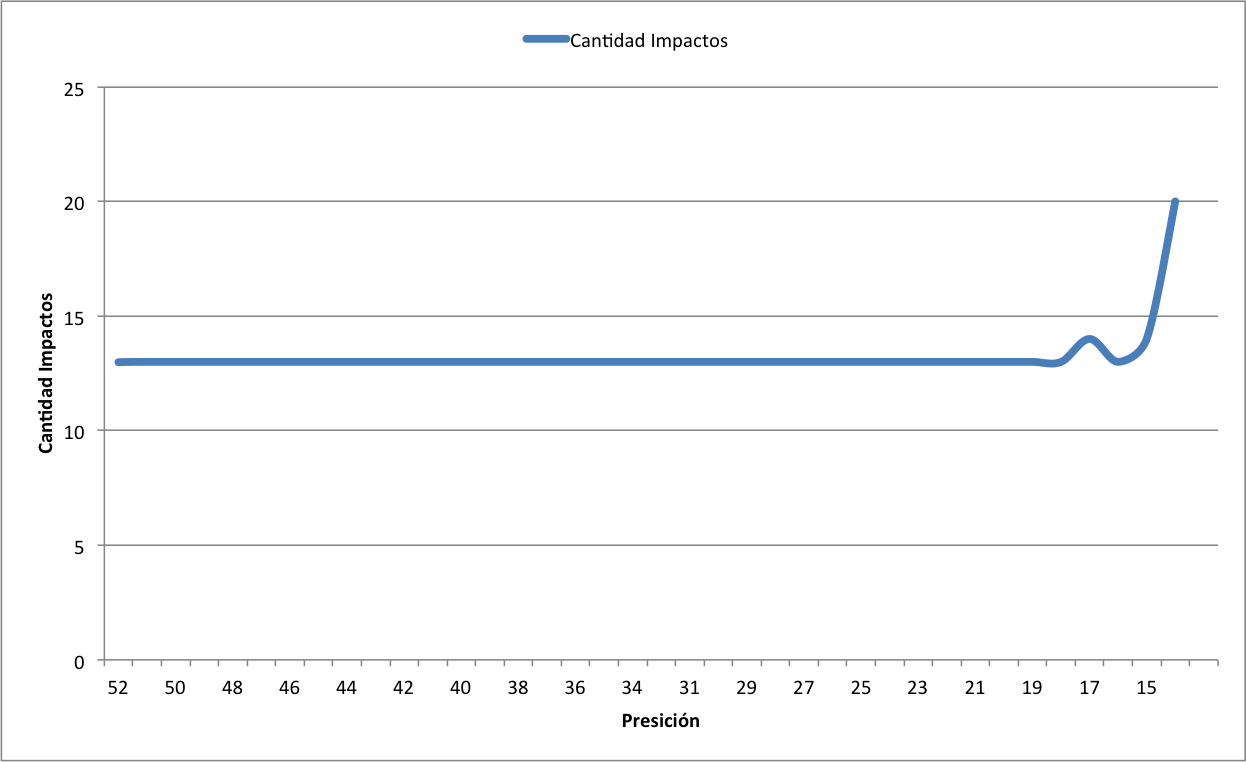
\includegraphics[scale=0.65]{graficos/extra-cantidad_impactos.png}
  \caption{Cantidad de impactos, variando la presición de 52 a 2.}
\end{figure}

\begin{figure}[H]
  \centering
  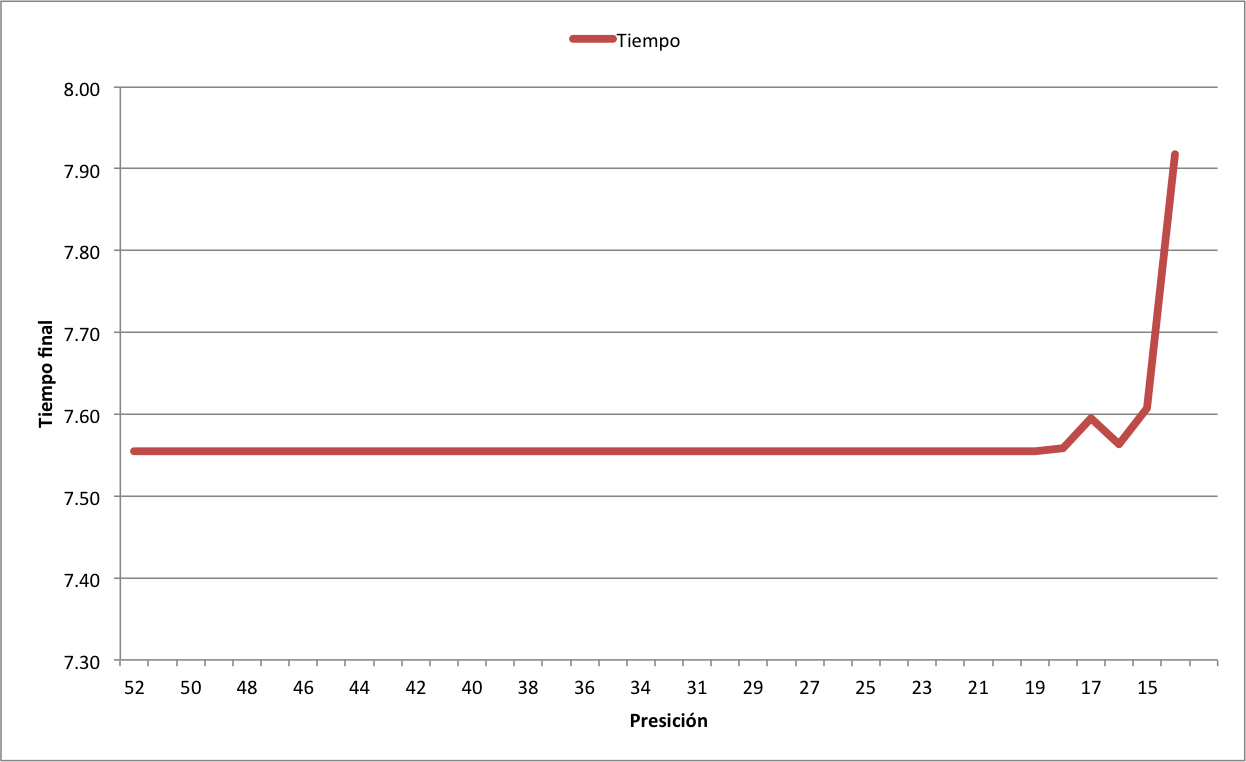
\includegraphics[scale=0.65]{graficos/extra-tiempo.png}
  \caption{Tiempo final, variando la presición de 52 a 2.}
\end{figure}



Como observación de los gráficos, no representamos las precisiones a partir del 14 hasta el 2 dado que el algoritmo no terminaba porque no llegaba nunca a cumplir la condición de corte. Y ademas el criterio de parada por iteraciones hacía que el gráfico sea desproporcional.

\section{Conclusión}
En conclusión, el utilizar pocos dígitos de representación, no afecta solo el resultado final, sino que los errores se van acumulando por las operaciones y se va arrastrando y creciendo. 

Con esto vemos la importancia de la precisión, ya que para un problema podemos encontrar la solución, o una muy diferente a la real, o bien no encontrarla.
Es muy importante la precisión que se esta utilizando y el error que se esta cometiendo.

\end{document}

